%QUESTIONS HERE
%<*mytag1>
\begin{questions}[resume,noitemsep,leftmargin=20mm,labelsep=0.1cm]
\item What does TACACS+ stand for, and what is it used for?
\item What is the difference between TACACS+ and TACACS?
\end{questions}
%</mytag1>

%<*mytag2>
\begin{questions}[resume,noitemsep,leftmargin=20mm,labelsep=0.1cm]
\item Provide 2 forms of proof that the TACACS+ server is up and running on the windows 7 vm.
\item What port does the tacacs.net tacacs+ server run on by default?
\item Show evidence that the tacacs+ server can be started and stopped with \texttt{net stop tacacs.net} and \texttt{net start tacacs.net} in an administrative terminal.
\end{questions}
%</mytag2>

%<*mytag3>
\begin{questions}[resume,start=\number\value{questionsi}+1,noitemsep,leftmargin=20mm,labelsep=0.1cm]
\item Verify that the list of configuration files include: authentication, authorization, clients, googleotp, and tacplus.
\end{questions}
%</mytag3>

%<*mytag4>
\begin{questions}[resume,start=\number\value{questionsi}+1,noitemsep,leftmargin=20mm,labelsep=0.1cm]
\item What do the -k, -u, and -p flags mean?
\item How are we able to execute the \texttt{tactest} on the user "checkout" if we did not manually set the user up?
\item Did the \texttt{tactest}s work? Provide screenshots for evidence.
\end{questions}
%</mytag4> 

%<*mytag5>
\begin{questions}[resume*,start=\number\value{questionsi}+1,noitemsep,leftmargin=20mm,labelsep=0.1cm]
\item Identify 5 different services that are reported by nmap. Provide for each the associated port number, OS, OS version, and whether the port is open/close.
\end{questions}
%</mytag5> 

%<*mytag6>
\begin{questions}[resume,start=\number\value{questionsi}+1,noitemsep,leftmargin=20mm,labelsep=0.1cm]
\item Provide a brief description/definition for each of the designations: critical, high, medium, low and info.  Provide an example of each from the Nessus run.
\end{questions}
%</mytag6> 

%<*mytag7>
\begin{questions}[resume*,start=\number\value{questionsi}+1,noitemsep,leftmargin=20mm,labelsep=0.1cm]
\item Provide detailed description of the Risk Information and the vulnerability information of this specific CVE
\item What does “Exploitable with Metasploit (Samba "username map script" Command Execution)” mean?
\item Click on the first item under the Reference Information (that is CVE-2007-2447) and provide a summary of what is presented under that CVE.  When was the CVE 2007 2447 released?
\end{questions}
%</mytag7>

%<*mytag8>
\begin{questions}[resume,start=\number\value{questionsi}+1,noitemsep,leftmargin=20mm,labelsep=0.1cm]
\item Identify the CVE numbers associated with these. One of them does not have a CVE number. Why? \hl{Hint: Use the following syntax search vulns |grep samba}
\item Find the metasploit exploits for the two vulnerabilities hl{with CVE numbers}.  Hint: search CVE-$<$integer$>$-$<$integer$>$.  Did you find Metasploit exploit for both?  If not, why?
\end{questions}
%</mytag8>

%<*mytag9>
\begin{questions}[resume,start=\number\value{questionsi}+1,noitemsep,leftmargin=20mm,labelsep=0.1cm]
\item Explain RCE, CVE, BID, OSVDB, CERT, MSF, and NSS. Make sure to provide a citation for each.
\end{questions}
%</mytag9>


%<*mytag10>
\begin{enumerate}[noitemsep,label=$\circ$,leftmargin=17mm,labelsep=0.5cm]
\item Lack of intergrity checking
\item Vulnerability to replay attacks
\item Forced session\textunderscore id collisions
\item The birthday paradox and session\textunderscore id's
\item Lack of padding
\item MD5 context leak
\item Packet body length DoS and/or overflow
\end{enumerate}
%</mytag10>

%<*mytag11>
\begin{enumerate}[noitemsep,leftmargin=10mm,labelsep=0.1cm]
\item 
\end{enumerate}
%</mytag11>


%COMMANDS HERE
%<*mytag12>
\begin{enumerate}[noitemsep,leftmargin=10mm,labelsep=0.1cm]
\item [] \textbf{python tacoflip.py -t 10.10.10.100 -v}
\end{enumerate}
%</mytag12>

%<*mytag13>
\begin{enumerate}[noitemsep,leftmargin=10mm,labelsep=0.1cm]
\item [] \textbf{ettercap -G}
\end{enumerate}
%</mytag13>
%<*mytag14>
\begin{enumerate}[noitemsep,label=$\circ$,leftmargin=17mm,labelsep=0.5cm]
\item \textbf{Configured Kali-Linux VM with at least 8 G of RAM and 4 processors}
\item Kali Linux and Metasploitable2-Linux VMs are up.
\item Nessus installed on Kali-Linux
\end{enumerate}
%</mytag14>
%<*mytag15>
\begin{enumerate}[noitemsep,leftmargin=10mm,labelsep=0.1cm]
\item [] \textbf{tactest -k testsecret -u testuser1 -p testpassword}
\item [] \textbf{tactest -k testsecret -u checkout -p checkout}
\end{enumerate}
%</mytag15>
%<*mytag16>
\begin{enumerate}[noitemsep,leftmargin=10mm,labelsep=0.1cm]
\item [] \textbf{msfconsole}
\end{enumerate}
%</mytag16>
%<*mytag17>
\begin{enumerate}[noitemsep,leftmargin=10mm,labelsep=0.1cm]
\item [] \textbf{db\_status}
\end{enumerate}
%</mytag17>
%<*mytag18>
\begin{enumerate}[noitemsep,leftmargin=10mm,labelsep=0.1cm]
\item [] \textbf{workspace}
\end{enumerate}
%</mytag18>
%<*mytag19>
\begin{enumerate}[noitemsep,leftmargin=10mm,labelsep=0.1cm]
\item [] \textbf{workspace –d $<$name of workspace$>$}
\end{enumerate}
%</mytag19>
%<*mytag20>
\begin{enumerate}[noitemsep,leftmargin=10mm,labelsep=0.1cm]
\item [] \textbf{workspace –a Group$<$your group number$>$-nmap}
\end{enumerate}
%</mytag20>
%<*mytag21>
\begin{enumerate}[noitemsep,leftmargin=10mm,labelsep=0.1cm]
\item [] \textbf{workspace Group$<$your group number$>$-nmap}
\end{enumerate}
%</mytag21>
%<*mytag22>
\begin{enumerate}[noitemsep,leftmargin=10mm,labelsep=0.1cm]
\item [] \textbf{db\_import} 
\end{enumerate}
%</mytag22>
%<*mytag23>
\begin{enumerate}[noitemsep,leftmargin=10mm,labelsep=0.1cm]
\item [] \textbf{hosts}
\end{enumerate}
%</mytag23>
%<*mytag24>
\begin{enumerate}[noitemsep,leftmargin=10mm,labelsep=0.1cm]
\item [] \textbf{services}
\end{enumerate}
%</mytag24>
%<*mytag25>
\begin{enumerate}[noitemsep,leftmargin=10mm,labelsep=0.1cm]
\item [] \textbf{vulns}
\end{enumerate}
%</mytag25>
%<*mytag26>
\begin{enumerate}[noitemsep,leftmargin=10mm,labelsep=0.1cm]
\item [] \textbf{db\_import $<$name of the Nessus scan file including path$>$}
\end{enumerate}
%</mytag26>
%<*mytag27>
\begin{enumerate}[noitemsep,leftmargin=10mm,labelsep=0.1cm]
\item [] \textbf{vulns}
\end{enumerate}
%</mytag27>
%<*mytag28>
\begin{enumerate}[noitemsep,label=$\circ$,leftmargin=14mm,labelsep=0.5cm]
\item Find Metasploit source code of the exploit CVE-2007-2447.  Find out the different payloads available, if any!  What programming language is it written in?  Provide a copy of the source code and explain what the code does.  Hint: it is a short script!
\item From the Wireshark capture in Step 2, find the specific set of packets exchanged between Nessus and Metasploitable2 that led Nessus to identify samba username vulnerability. Provide a pcap export of these packets and explain the algorithm used. 
\item \hl{Clone Nexpose VM (this is an open source equivalent to Nessus) and generate a vulnerability report on Metasploitable2.  Compare the results of Nessus and Nexpose in terms of the number of and the specific vulnerabilities identified.}
\end{enumerate}
%</mytag28>


%<*mytag29>
\begin{enumerate}[noitemsep,leftmargin=10mm,labelsep=0.1cm]
\item [] \textbf{len = TAC\_PLUS\_HDR\_SIZE + ntohl(hdr.datalength);}
\end{enumerate}
%</mytag29>

%<*mytag30>
\begin{questions}[resume,start=\number\value{questionsi}+1,noitemsep,leftmargin=20mm,labelsep=0.1cm]
\item What does the len variable represent? (No need to be overly technical)
\end{questions}
%</mytag30>

%<*mytag31>
\begin{enumerate}[noitemsep,leftmargin=10mm,labelsep=0.1cm]
\item [] \textbf{pkt = (u\_char *)tac\_malloc(len);}
\end{enumerate}
%</mytag31>

%<*mytag32>
\begin{enumerate}[noitemsep,leftmargin=10mm,labelsep=0.1cm]
\item [] \textbf{dpkg -s scapy}
\end{enumerate}
%</mytag32>

%<*mytag33>
\begin{enumerate}[noitemsep,leftmargin=10mm,labelsep=0.1cm]
\item [] \textbf{chmod 755 tacacs\_scapy.py}
\end{enumerate}
%</mytag33>

%<*mytag34>
\begin{enumerate}[noitemsep,leftmargin=10mm,labelsep=0.1cm]
\item [] \textbf{tac=Tacacs()}
\item [] \textbf{tac.display()}
\end{enumerate}
%</mytag34>

%<*mytag35>
\begin{questions}[resume,start=\number\value{questionsi}+1,noitemsep,leftmargin=20mm,labelsep=0.1cm]
\item Why did we need the script to examine a Tacacs+ packet with scapy? Hint: Look online for a list of protocol layers that scapy knows by default.
\end{questions}
%</mytag35>

%GRAPHICS HERE

%<*mtag1>
\begin{figure}[H]
\centering
\captionsetup{width=.8\linewidth}
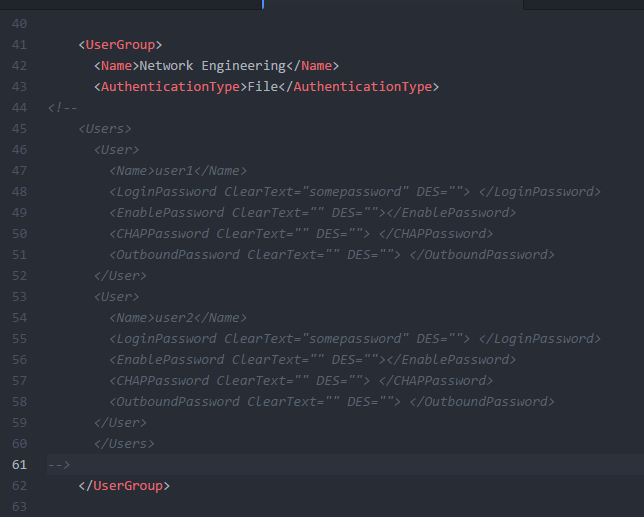
\includegraphics[scale=0.9]{img/8_commentusers.PNG}
\caption{}
\label{fig:users}
\centering
\end{figure}
%</mtag1>